\entry{Semana del 22/09/2025.} 

\section{Lunes 22/09/2025.} 

\subsection*{Prueba de usar la DAQ con varios canales.} 

Hoy empecé probando si el código de la interfaz de adquisición, tal cual estaba escrito, funcionaría bien para realizar una adquisición con más de dos canales como veníamos haciendo, en vista de la inminente utilización de múltiples sensores. 

Puse en los canales 0, 1 y 2 (en modo diferencial) de la DAQ la misma señal del generador de funciones (una sinoidal de frecuencia 52.676 kHz y amplitud 10 Vpp) y medí durante 1 segundo a la máxima frecuencia de sampleo de la placa (1 MHz). 

\begin{figure}[th!]
	\centering
	\includegraphics[width=0.2731241567\linewidth]{"Figures/22_09_2025/Conexiones placa"}
	\caption{Conexiones de los tres canales de la placa DAQ.}
	\label{fig:conexiones-placa} 
\end{figure}


El resultado fue una medición a 333.333 kHz en cada uno de los tres canales (un millón de puntos en total) y el voltaje registrado fue el siguiente: 

\begin{figure}[th!]
	\centering
	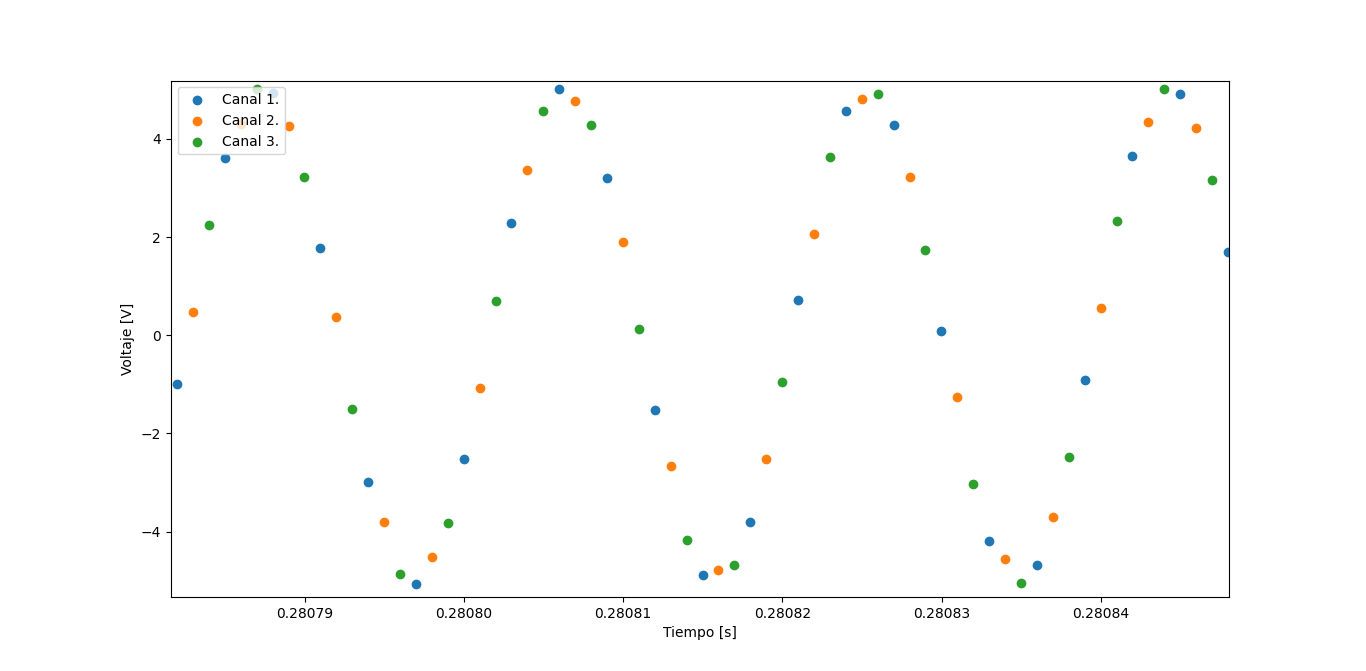
\includegraphics[width=0.87\linewidth]{Figures/22_09_2025/Prueba_con_3_canales}
	\caption{Medición en los tres canales de la DAQ de la misma señal de referencia.}
	\label{fig:pruebacon3canales}
\end{figure} 

Como se puede notar de la Figura en efecto los tres canales están midiendo la misma señal (con el retardo de 1 $\mu$s de cada uno) que pareciera tener las características de amplitud y frecuencia esperadas. 


\subsection*{Pruebas con dos sensores.} % n 
Voy a empezar a hacer pruebas usando dos sensores en simultáneo. Un par de cosas que noté al esmaltar el segundo sensor: 

\begin{itemize}
	\item El grosor del esmaltado de cobre puede variar cerca de la punta, si esa es la sección sumergida podemos tener un $\varepsilon(l)$ afectando la relación lineal. 
	\item Se esmalta también parte del alambre de acero, lo que puede hacer que no se ponga bien a Tierra el agua. Cosas que se podrían hacer es raparlo con el alicate o con fuego para sacar ese nuevo esmalte. También se podría intentar esmaltarlo completamente a propósito y ver como afecta. Igualmente imagino que si está lo suficientemente sumegido como para llegar a la parte que no se esmaltó debería estar bien.  
\end{itemize}

Ya tengo todo montado, quedó bastante compacto. Más abajo detalle de la disposición de los sensores y la paleta del motor y de las conexiones de la ProtoBoard por las dudas.  % b 

\begin{figure}[!ht]
	\begin{minipage}[c]{0.5\textwidth}
		\begin{subfigure}{\textwidth}
			\centering
			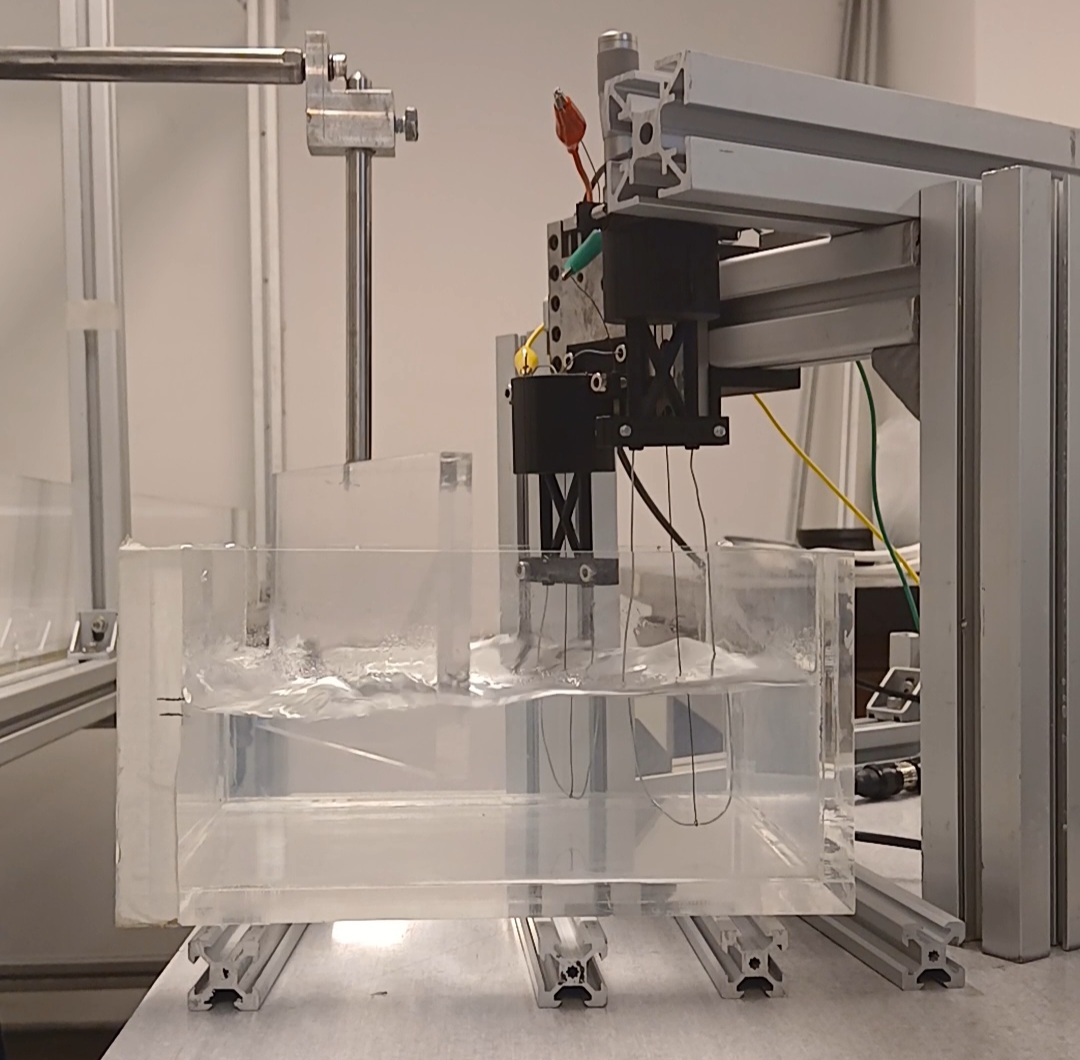
\includegraphics[width=0.958\textwidth]{Figures/22_09_2025/Setup montaje.jpg}
			\captionsetup{width=0.8\textwidth}
			\subcaption{Sensores sumergidos.}
			% \label{fig:}
		\end{subfigure}
	\end{minipage}\begin{minipage}[c]{0.49\textwidth}
		\begin{subfigure}{\textwidth}
			\centering
			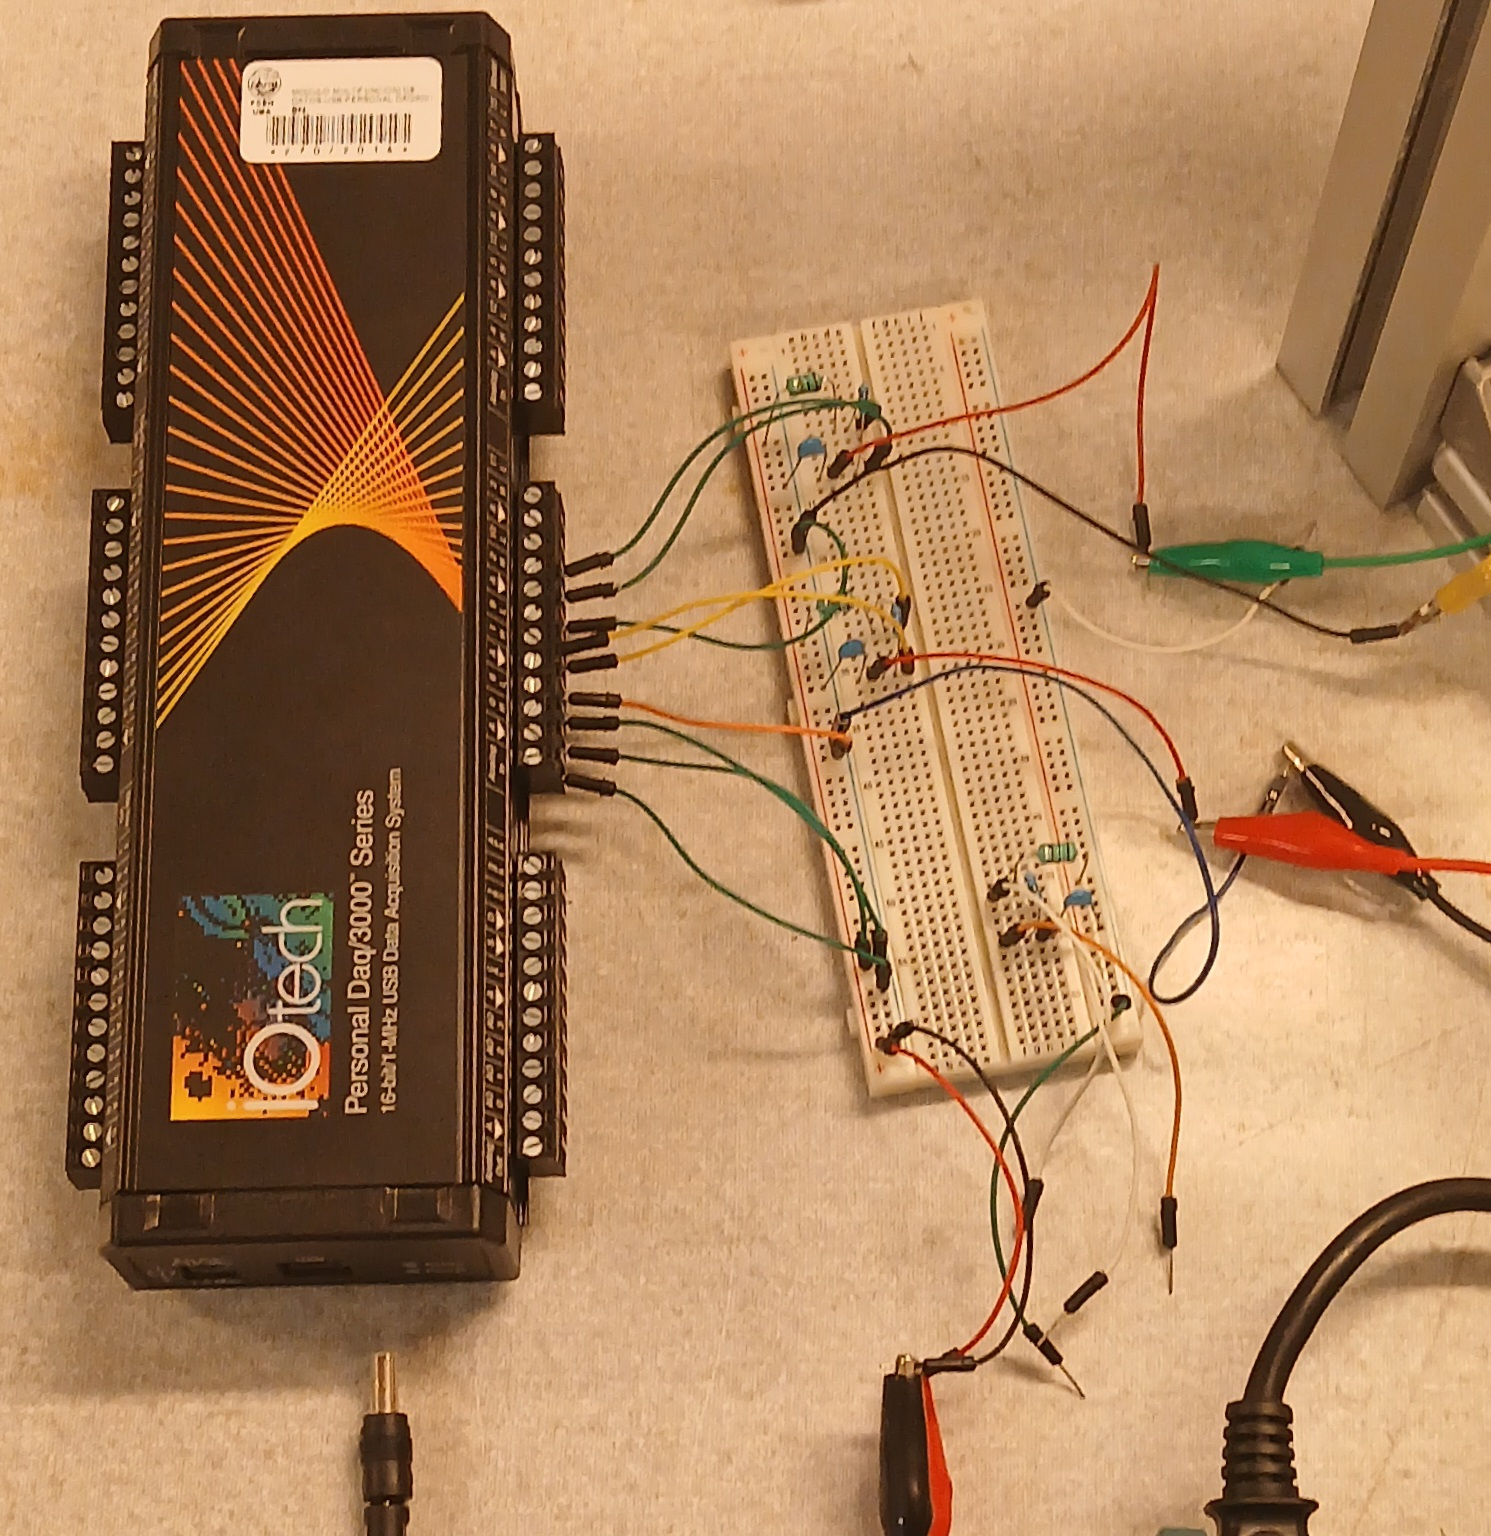
\includegraphics[width=0.958\textwidth]{Figures/22_09_2025/Conexiones montaje.jpg} 
			\captionsetup{width=0.8\textwidth} 
			\subcaption{Conexiones.}
			% \label{fig:}
		\end{subfigure}
	\end{minipage}
	\caption{Montaje experimental para la prueba de utilización de dos sensores en el montaje de turbulencia de ondas.} 
	\label{fig:montaje_dos_sensores_cuba_chica}
\end{figure}

Para tener en cuenta algunos detalles de mientras fui armando todo: 

\begin{itemize}
	\item Estoy usando para los dos circuitos RLC nuevos componentes (de valores R=360 $\Omega$, L=10 mH y C=560 pF como veníamos usando). 
	\item Tengo conectado el sensor nuevo al canal uno con los cables BNC largos y el sensor viejo al canal 2 con dos cablecitos cocodrilo-cocodrilo de 30 cm de largo, que limitan la disposición de los cables cómodamente. 
	\item El cable que conecta a Tierra al sensor viejo (2) tiene la cabeza del lado de la ProtoBoard rota, así que no sé que tan bien hará contacto. Igualmente si está el agua a Tierra con el otro sensor entiendo que debería ser suficiente. 
	\item La distancia entre los dos alambres de cobre es de 8 cm aproximadamente (medido en lo más alto del sensor 2 que es el que está más bajo). 
	\item Al no usar el perfil largo que se agarra de arriba y de abajo el motor vibra mucho al moverse, por lo menos con la cuba vacía. 
	\item Mantengo en el generador de funciones los 52.676 kHz y 10 Vpp. 
\end{itemize} 

Para poder normalizar las señales y que no haya constantes dando vueltas a la hora de hacer la correlación (sino después normalizar con la raíz de la autocorrelación cuadrada) voy a tomar dos mediciones de la superficie estática en alturas distintas mientras lleno. 



Los puntos de referencia durante el llenado fueron 4.05 cm de la altura 1 (esta no estoy 100 \% seguro y tomé solo dos canales). 5.05 cm altura 2 y 5.50 cm para la altura 3 (Habría que usar estas dos). Para la 3 llené un poco más usando el vaso de precipitados de plástico. 

Voy a tomar mediciones para las curvas de las bandas entre 0-4 Hz  y  0-6 Hz, ambas con 50 \% de la amplitud total para que sea comparable a lo anterior. Los sensores están ambos con la parte más baja casi en el piso (alineé el del tornillo para qe queden a la misma altura las bases). 

Mientras iba llenando noté en la interfaz de tiempo real que al irse sumergiendo el nuevo sensor efectivamente hizo cosas raras al principio (poco sumergido) pero después se estabilizó y dio una disminución de la fase (aumento de la altura) más o menos lineal con el llenado con la manguera. 

Tuve que aumentar al triple el buffer circular porque sino había overrun. 

Me estoy llevando también por las dudas la posición real del motor durante un intervalo de 60 segundos durante la medición. 

La amplitud de las ondas es de más o menos 1 cm, no sé que tan bien valdrá la aproximación de profundidad finita para llenado de 5.5 cm.   

Por último me parece que me voy a llevar la medición del homing para tratar de caracterizar en qué orden de frecuencias son las vibraciones del motor. El inicio antes del homing me sirve como medida del ruido de ambos sensores también.   


\subsection*{Análisis de los datos.} 
El sensor original (que estaba con el cable malo y en el canal 2) parece estar funcionando bien, mientras que el nuevo me da básicamente ruido. No estoy del todo seguro si es que se desconectó algún cable o hay alguna otra cosa detrás, como que al ser más largo la frecuencia de resonancia es muy distinta y se sale del rango de medición. Ahora voy a probar de nuevo con el graficador en tiempo real. 

Me parece igualmente que al sensor viejo le pudo haber pasado algo ya que ahora las mediciones son bastante más ruidosas que antes. 

Me acabo de dar cuenta que el retraso fraccional ya no va a ser de medio punto sino de 1/3 y 2/3. Igualmente eso debería agregar una fase constante en cualquier caso. 

Ahhhh, estoy usando en el análisis \textit{channel-1} pero sería simplemente \textit{channel} ya que el 0 es la referencia, el que da ruido es referencia contra referencia entonces y el que daba bien es el sensor nuevo. 

Habría que implementar el graficador en tiempo real para N sensores para poder verificar antes de medir si está andando correctamente. Más allá de eso parece que sí está funcionando. 

\subsection*{Resultados del forzado en 0-6 Hz.} 
De momento lo que hice fue ver las series temporales de cada uno y calcular la PSD con Welch. Los  resultados son los que están más abajo. 

\begin{figure}[th!]
	\centering
	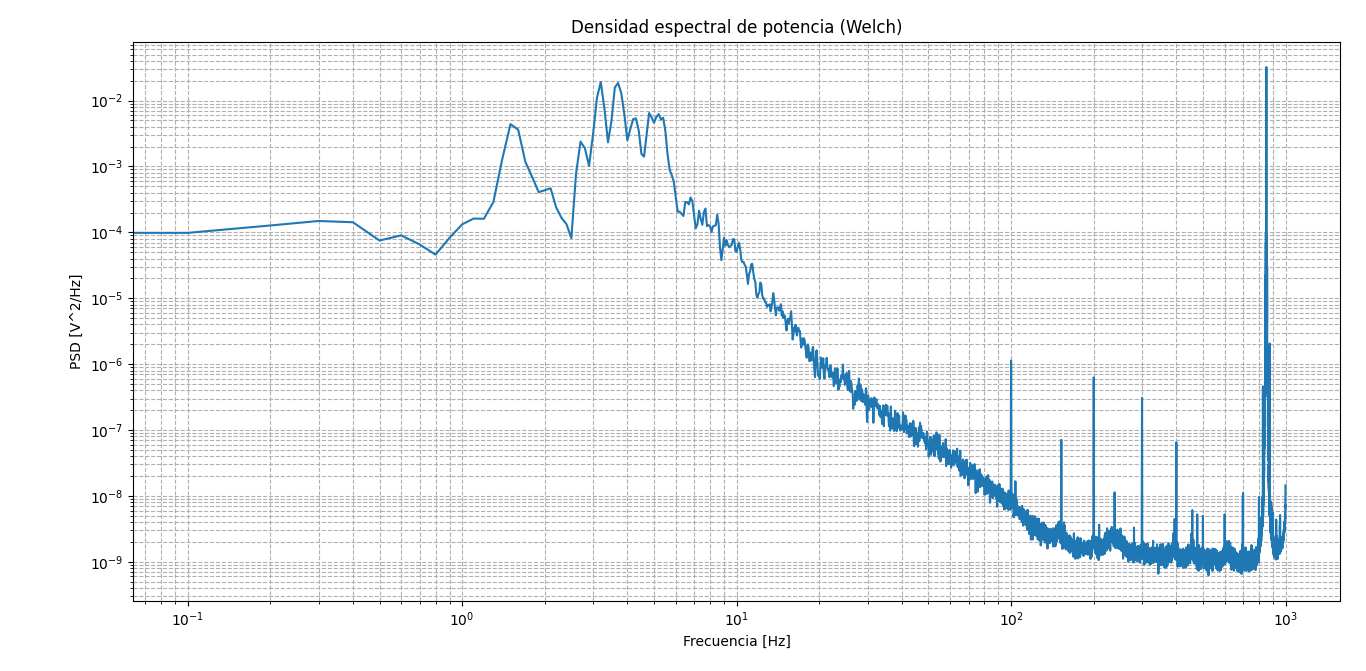
\includegraphics[width=0.87\linewidth]{Figures/22_09_2025/Espectro_0_6_Hz_sensor_viejo} 
	
	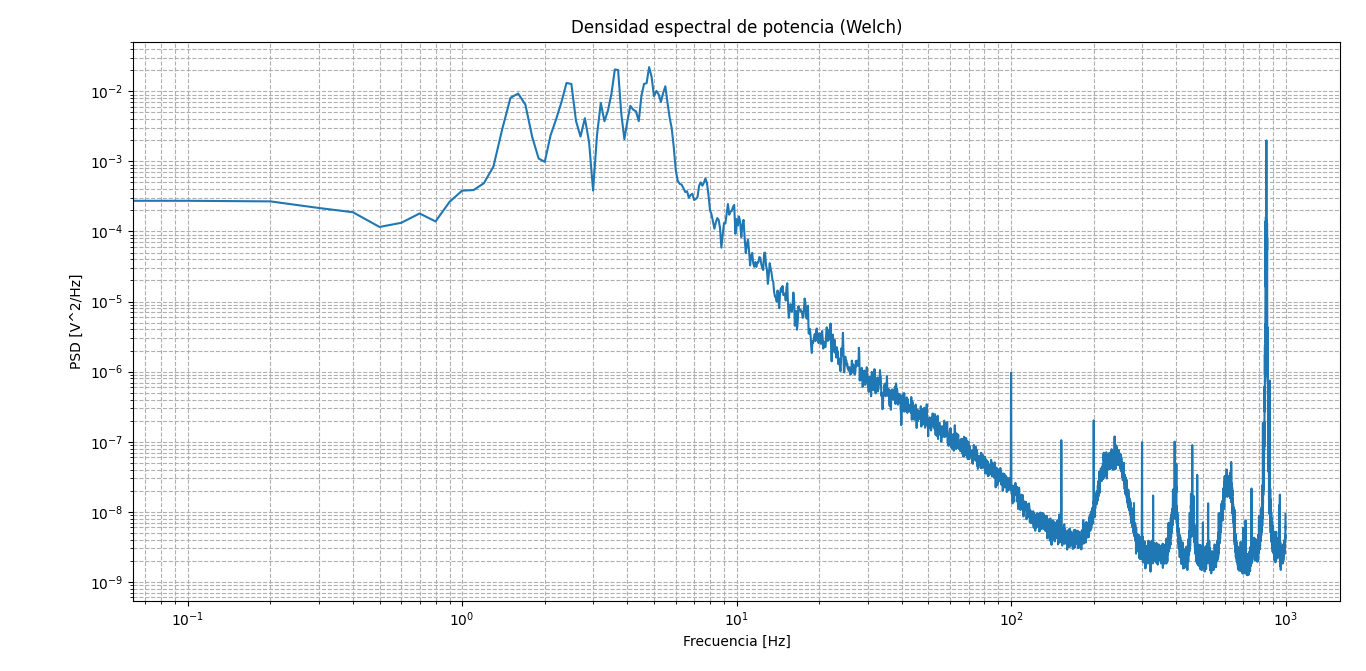
\includegraphics[width=0.87\linewidth]{Figures/22_09_2025/Espectro_0_6_Hz_sensor_nuevo}
	\caption{Arriba espectro de la señal del sensor viejo y abajo la del sensor nuevo (con todos los mismos parámetros que el análisis original).}
	\label{fig:espectro06hz_dos_sensores}
\end{figure}

Ambos espectros son razonablemente similares como esperaríamos. La diferencia principal está en las oscilaciones en frecuencias altas (más altas que la de corte). Para el sensor viejo están presentes pero con mucha menor amplitud. 

Estas oscilaciones estaban en las mediciones anteriores para la banda de 0-5 Hz (Miércoles 27/08/2025). 

Una posible explicación sería que se acoplen al movimiento de la superficie oscilaciones del alambre de acero o cobre (al estilo de una cuerda de piano) ya que son frecuencias muy altas. Habría que estimar cuánta tensión sería necesaria para que la frecuencia fundamental sea la del pico mayor que aparece aproximadamente en 245 Hz y determinar si sería algo razonable (para después plantearnos si vale la pena medir bien esa tensión). 

Además resta calcular la correlación entre ambas señales. Deberíamos esperar ver una réplica luego de un tiempo correspondiente al de viaje de una onda de la frecuencia fundamental (tipo 4 Hz el pico principal) en la distancia entre alambres (de 8 cm). Esperaríamos que en esa distancia no afecten tanto los efectos dispersivos.    


\section{Miércoles 24/09/2025.} 

Un par de cosas que quedaron pendientes revisar la vez pasada. Por un lado las señales de cada sensor, normalizadas por la desviación estándar y sin media. % : 

\begin{figure}[th!]
	\centering
	\includegraphics[width=0.765\linewidth]{"Figures/22_09_2025/Señales temporales v2"}
	\caption{Señales de los dos sensores.}
	\label{fig:senales-temporales}
\end{figure}

Para esto subsamplee la señal a un quinto de los puntos, ya que sino tenía bastante ruido (supongo por los picos raros a frecuencias altas, que de momento por las estimaciones darían tensiones del orden de 0.1-1 N que parecen consistentes). La señal del sensor nuevo pareciera ser un poco más ruidosa tal vez. 

 

Además las PDFs que siguen dando como deberían: 

\begin{figure}[th!]
	\centering
	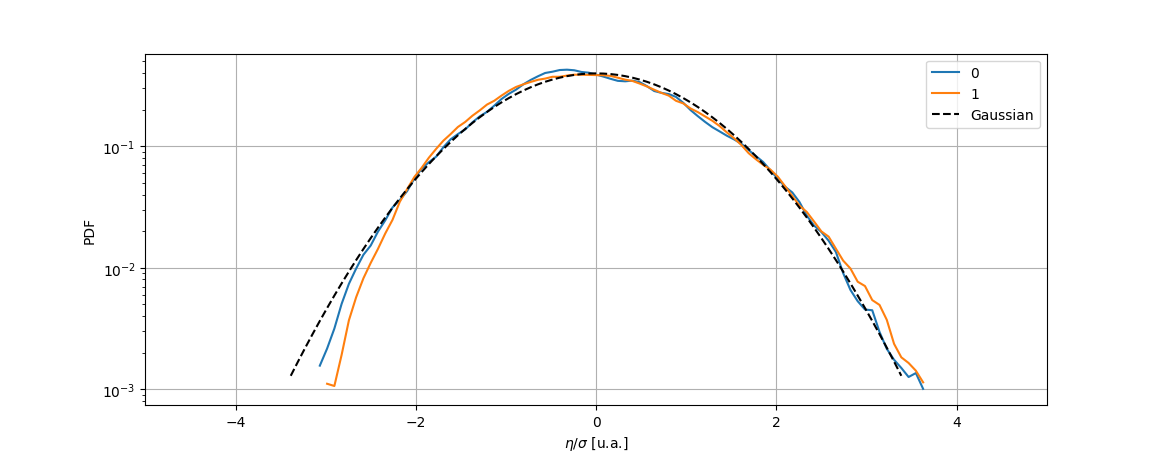
\includegraphics[width=0.7\linewidth]{Figures/22_09_2025/PDFS_sensores_0_6_Hz}
	\caption{PDFS de las señales de los dos sensores.}
	\label{fig:pdfssensores06hz}
\end{figure}

\subsection*{Correlación cruzada entre sensores.} 
Lo que hice acá fue tomar una ventana de la señal del primer sensor $h_1$ y calcular su correlación con otra más larga de $h_2$, ambas arrancando en el mismo punto. Después fui moviendo las ventanas manteniendo su longitud constante y asegurándome que empiecen siempre en el mismo índice y calculé el promedio de todas esas correlaciones, que es lo siguiente: 

\begin{figure}[th!]
	\centering
	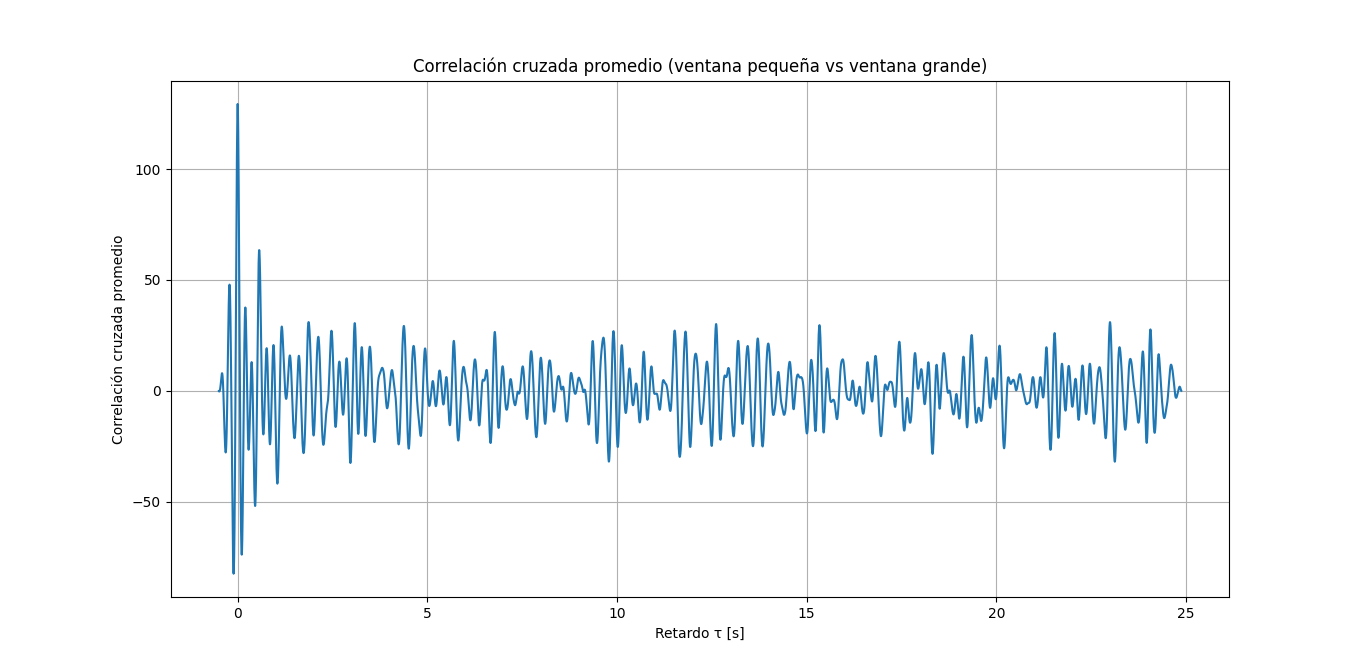
\includegraphics[width=0.87\linewidth]{Figures/22_09_2025/Correlación_ventana_h1_vs_h2}
	\caption{Correlación de $h_1$ vs $h_2$.}
	\label{fig:correlacionventanah1vsh2}
\end{figure}

Hay un pico cuando el desfasaje entre señales es 0 y después otro más pequeño a los 0.57 s que podría ser de una onda que viaja entre ambos sensores. 

 
  
  
  